\documentclass{article}

\usepackage[linesnumbered,lined,boxed,commentsnumbered]{algorithm2e}
\usepackage[dvipsnames]{xcolor}
\usepackage{tikz}
\usepackage{subcaption}
\usetikzlibrary{arrows,automata,matrix,chains,positioning,decorations.pathreplacing,arrows}

\begin{document}

\section{Algorithmus}
\begin{algorithm}
	
	\caption{Gradient descent}
	\KwIn{loss function $E$, learning rate $\eta$, dataset $ X, y $ und das Modell $ F(\theta, x) $}
	\KwOut{Optimum $\theta$ which minimizes $\epsilon$ }
	\DontPrintSemicolon
	
	\While{converge}{
		$\tilde{y}= F(\theta, x)$\;
		$\theta = \theta -\eta.\frac{1}{N}\sum_{i=1}^{N}\frac{\delta\epsilon(y,\tilde{y})}{\delta\theta}$\;

	}
	\label{algo:GD}
\end{algorithm}


\begin{algorithm}
	\caption{Stochastic Gradient descent(SGD)}
	\KwIn{loss function $E$, learning rate $\eta$, dataset $ X, y $ und das Modell $ F(\theta, x) $}
	\KwOut{Optimum $\theta$ which minimizes $\epsilon$ }
	\DontPrintSemicolon
	
	\While{converge}{
		Shuffle X, y\;
		\For{ $ x_i, y_i $ in X, y}{
		$\tilde{y}= F(\theta, x_i)$\;
		
		$\theta = \theta -\eta.\frac{1}{N}\sum_{i=1}^{N}\frac{\delta\epsilon(y_i,\tilde{y_i})}{\delta\theta}$\;
	}
		
	}
	\label{algo:SGD}
\end{algorithm}

\begin{algorithm}
	\caption{Mini-Batch Stochastic Gradient descent(MSGD)}
	\KwIn{loss function $E$, learning rate $\eta$, dataset $ X, y $ und das Modell $ F(\theta, x) $}
	\KwOut{Optimum $\theta$ which minimizes $E$ }
	\DontPrintSemicolon
	
	\While{converge}{
		Shuffle X, y\;
		\For{each batch of $ x_i, y_i $ in X, y}{
			$\tilde{y}= F(\theta, x_i)$\;
			
			$\theta = \theta -\eta.\frac{1}{N}\sum_{i=1}^{N}\frac{\delta E(y_i,\tilde{y_i})}{\delta E}$\;
		}
		
	}
	\label{algo:MSGD}
\end{algorithm}
\newpage
\begin{algorithm}
	\caption{Back-Propagation}
	\KwIn{Netzwerk mit $ l $ layers, Aktivirungsfunktion $\sigma_l$ , Output von der verstekten Schicht $ h_l =\sigma_l(W_l^Th_{l-1} +b_{l}) $  und die Netzwerkausgabe $\tilde{y}= h_{l}$}
	\DontPrintSemicolon
	Berechnen der Gradient: $\delta \gets \frac{\partial E(y_{i}, \tilde{y}_i)}{\partial y}$ \;
	\For{$ i \gets l $ bis $ 0 $ }{
		Berechnen der Gradient für die Aktuelle Schicht \;
		$\frac{\partial E(y, \tilde{y})}{\partial W_l} =\frac{\partial E(y, \tilde{y})}{\partial h_l}\frac{\partial h_l}{\partial W_l} = \delta\frac{\partial h_l}{\partial W_l}$\;
			$\frac{\partial E(y, \tilde{y})}{\partial b_l} =\frac{\partial E(y, \tilde{y})}{\partial h_l}\frac{\partial h_l}{\partial b_l} = \delta\frac{\partial h_l}{\partial b_l}$\;
		
	   Gradientabstiegverfahren mit 	$ \frac{\partial E(y, \tilde{y})}{\partial W_l} $ und $ \frac{\partial E(y, \tilde{y})}{\partial b_l} $\;
	   Propagiere den Gradienten zu den unteren Schichten.\;
	   $\delta \gets \frac{\partial E(y, \tilde{y})}{\partial h_l}\frac{\partial h_l}{\partial h_{l-1}} = \delta \frac{\partial h_l}{\partial h_{l-1}}$\;
		
	}
	\label{algo:BP}
\end{algorithm}

\section{Neuronale Netzwerk}
\begin{figure}[h!]
	\centering
	\begin{subfigure}{\textwidth}
		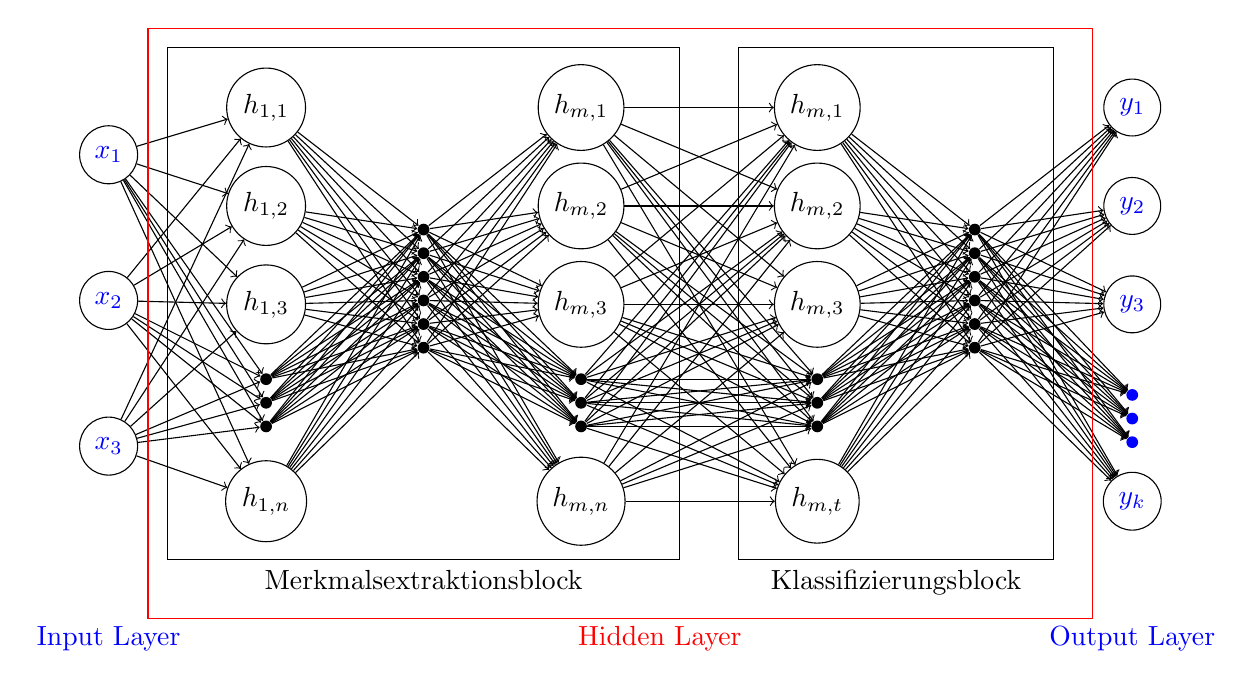
\begin{tikzpicture}
		\tikzstyle{place}=[circle, draw=black, minimum size = 5mm]
		
		% Input
		\foreach \x in {1,...,3}
		\draw node[text=blue] at (0, -\x*1.85) [place] (first_\x) {$x_\x$};
		
		% Hidden 1
		\foreach \x in {1,...,3}
		\node[text=black] at (2, -\x*1.25) [place] (h1_\x){$h_{1,\x}$};
		\foreach \x in {4,...,6}
		\node[circle, fill=black,minimum size=2pt, inner sep=1.5, label={}] (h1_\x) at (2, -3.5 -\x*0.3) {};
		\draw node[text=black] at (2, -5*1.25) [place] (h1_n) {$h_{1, n}$};
		
		% Hidden 2
		\foreach \x in {1,...,6}
		\node[circle, fill=black,minimum size=2pt, inner sep=1.5, label={}] (h2_\x) at (4, -2.5 -\x*0.3) {};
		
		
		% Hidden 3
		\foreach \x in {1,...,3}
		\node[text=black] at (6, -\x*1.25) [place] (h3_\x){$h_{m, \x}$};
		\foreach \x in {4,...,6}
		\node[circle, fill=black,minimum size=2pt, inner sep=1.5, label={}] (h3_\x) at (6, -3.5 -\x*0.3) {};
		\draw node[text=black] at (6, -5*1.25) [place] (h3_n) {$h_{m, n}$};
		
		
		
		% Hidden 4
		\foreach \x in {1,...,3}
		\node[text=black] at (9, -\x*1.25) [place] (h4_\x){$h_{m, \x}$};
		\foreach \x in {4,...,6}
		\node[circle, fill=black,minimum size=2pt, inner sep=1.5, label={}] (h4_\x) at (9, -3.5 -\x*0.3) {};
		\draw node[text=black] at (9, -5*1.25) [place] (h4_n) {$h_{m, t}$};
		
		% Hidden 5
		\foreach \x in {1,...,6}
		\node[circle, fill=black,minimum size=2pt, inner sep=1.5, label={}] (h5_\x) at (11, -2.5 -\x*0.3) {};
		
		
		% Output
		\foreach \x in {1,...,3}
		\node[text=blue] at (13, -\x*1.25) [place] (output_\x){$y_\x$};
		\foreach \x in {4,...,6}
		\node[circle, fill=blue,minimum size=2pt, inner sep=1.5, label={}] (output_\x) at (13, -3.7 -\x*0.3) {};
		\node[text=blue] at (13, -5*1.25) [place] (output_n) {$y_k$};
		
		% Input -> Hidden 1
		\foreach \i in {1,...,3}
		\foreach \j in {1,...,6}
		\draw [->] (first_\i) to (h1_\j);
		\foreach \i in {1,...,3}
		\draw [->] (first_\i) to (h1_n);
		%		\foreach \i in {1,...,3}
		%		\draw [->] (first_n) to (second_\i);
		%		\draw [->] (first_n) to (second_m);
		
		% Hidden 1 -> Hidden 2
		\foreach \i in {1,...,6}
		\foreach \j in {1,...,6}
		\draw [->] (h1_\i) to (h2_\j);
		\foreach \i in {1,...,6}
		\draw [->] (h1_n) to (h2_\i);
		
		% Hidden 2 -> Hidden 3
		\foreach \i in {1,...,6}
		\foreach \j in {1,...,6}
		\draw [->] (h2_\i) to (h3_\j);
		\foreach \i in {1,...,6}
		\draw [->] (h2_\i) to (h3_n);
		
		% Hidden 3 -> Hidden 4
		\foreach \i in {1,...,6}
		\foreach \j in {1,...,6}
		\draw [->] (h3_\i) to (h4_\j);
		\foreach \i in {1,...,6}
		\draw [->] (h3_n) to (h4_\i);
		\foreach \i in {1,...,6}
		\draw [->] (h3_\i) to (h4_n);
		\draw [->] (h3_n) to (h4_n);
		
		% Hidden 4 -> Hidden 5
		\foreach \i in {1,...,6}
		\foreach \j in {1,...,6}
		\draw [->] (h4_\i) to (h5_\j);
		\foreach \i in {1,..., 6}
		\draw [->] (h4_n) to (h5_\i);
		
		
		% Hidden 5 -> Output
		\foreach \i in {1,...,6}
		\foreach \j in {1,...,6}
		\draw [->] (h5_\i) to (output_\j);
		\foreach \i in {1,...,6}
		\draw [->] (h5_\i) to (output_n);
		
		% Text
		\node at (0, -8) [blue, ] {Input Layer};
		\node at (7, -8) [red, ] {Hidden Layer};
		\node at (13, -8) [blue, ] {Output Layer};
		%Rectangle
		%		\draw[draw=black, label=below:stack, inner sep=0pt] (1,-7) -- (7,-7) -- (7,-0.5) -- (1,-0.5) -- cycle;
		\node at (4,-7) [draw=black,name=A,rectangle, minimum width=6.5cm,minimum height=6.5cm,anchor=south,label=below:Merkmalsextraktionsblock,transform shape] {};
		\node at (10,-7) [draw=black,text=Cerulean, name=A,rectangle, minimum width=4cm,minimum height=6.5cm,anchor=south,label=below:Klassifizierungsblock,transform shape] {};
		\node at (6.5,-7.75) [draw=red, name=A,rectangle, minimum width=12cm,minimum height=7.5cm,anchor=south,transform shape] {};
		
		\end{tikzpicture}
		\caption{\textit{TemkiNet Architektur}}
	\end{subfigure}	%
	\begin{subfigure}{\textwidth}
			\centering
	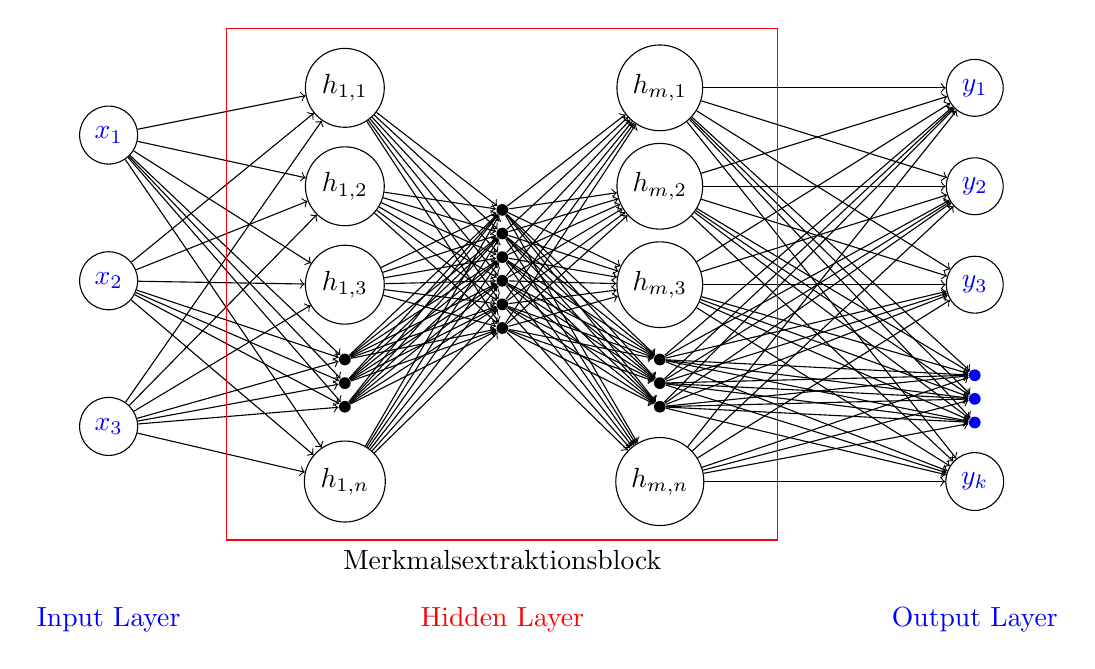
\begin{tikzpicture}
		\tikzstyle{place}=[circle, draw=black, minimum size = 5mm]
		
		% Input
		\foreach \x in {1,...,3}
		\draw node[text=blue] at (0, -\x*1.85) [place] (first_\x) {$x_\x$};
		
		% Hidden 1
		\foreach \x in {1,...,3}
		\node[text=black] at (3, -\x*1.25) [place] (h1_\x){$h_{1,\x}$};
		\foreach \x in {4,...,6}
		\node[circle, fill=black,minimum size=2pt, inner sep=1.5, label={}] (h1_\x) at (3, -3.5 -\x*0.3) {};
		\draw node[text=black] at (3, -5*1.25) [place] (h1_n) {$h_{1, n}$};
		
		% Hidden 2
		\foreach \x in {1,...,6}
		\node[circle, fill=black,minimum size=2pt, inner sep=1.5, label={}] (h2_\x) at (5, -2.5 -\x*0.3) {};
		
		
		% Hidden 3
		\foreach \x in {1,...,3}
		\node[text=black] at (7, -\x*1.25) [place] (h3_\x){$h_{m, \x}$};
		\foreach \x in {4,...,6}
		\node[circle, fill=black,minimum size=2pt, inner sep=1.5, label={}] (h3_\x) at (7, -3.5 -\x*0.3) {};
		\draw node[text=black] at (7, -5*1.25) [place] (h3_n) {$h_{m, n}$};
		
		% Output
		\foreach \x in {1,...,3}
		\node[text=blue] at (11, -\x*1.25) [place] (output_\x){$y_\x$};
		\foreach \x in {4,...,6}
		\node[circle, fill=blue,minimum size=2pt, inner sep=1.5, label={}] (output_\x) at (11, -3.7 -\x*0.3) {};
		\node[text=blue] at (11, -5*1.25) [place] (output_n) {$y_k$};
		
		% Input -> Hidden 1
		\foreach \i in {1,...,3}
		\foreach \j in {1,...,6}
		\draw [->] (first_\i) to (h1_\j);
		\foreach \i in {1,...,3}
		\draw [->] (first_\i) to (h1_n);
		%		\foreach \i in {1,...,3}
		%		\draw [->] (first_n) to (second_\i);
		%		\draw [->] (first_n) to (second_m);
		
		% Hidden 1 -> Hidden 2
		\foreach \i in {1,...,6}
		\foreach \j in {1,...,6}
		\draw [->] (h1_\i) to (h2_\j);
		\foreach \i in {1,...,6}
		\draw [->] (h1_n) to (h2_\i);
		
		% Hidden 2 -> Hidden 3
		\foreach \i in {1,...,6}
		\foreach \j in {1,...,6}
		\draw [->] (h2_\i) to (h3_\j);
		\foreach \i in {1,...,6}
		\draw [->] (h2_\i) to (h3_n);
		
		
		% Hidden 3 -> Output
		\foreach \i in {1,...,6}
		\foreach \j in {1,...,6}
		\draw [->] (h3_\i) to (output_\j);
		\foreach \i in {1,...,6}
		\draw [->] (h3_\i) to (output_n);
		\foreach \i in {1,..., 6}
		\draw [->] (h3_n) to (output_\i);
		\draw [->] (h3_n) to (output_n);
		% Text
		\node at (0, -8) [blue, ] {Input Layer};
		\node at (5, -8) [red, ] {Hidden Layer};
		\node at (11, -8) [blue, ] {Output Layer};
		\node at (5,-7) [draw=red,name=A,rectangle, minimum width=7cm,minimum height=6.5cm,anchor=south,label=below:Merkmalsextraktionsblock,transform shape] {};
		\end{tikzpicture}
	\caption{Allgemeine CNN-Architektur}
	\label{fig:Allgemeine CNN-Architektur.}
	\end{subfigure}
	
\end{figure}
% End of code
\end{document} 
